\section{Simulations}
\label{sec:simulations}

We evaluate whether the locally popular and locally stable outcomes found by
\alglocpop\ and \alglocstab\ recover meaningful latent structure, rather than
only satisfying their game-theoretic termination conditions.  The experiments
cover two complementary tasks: community detection in networks and clustering
of vector data.  We compare against standard task-specific methods, examine the
effect of the FEN preference domain, relation thresholds, and initialization,
and report both agreement with reference labels and an internal,
label-independent quality measure.  The complete sweep contains 5,000 recorded
runs, of which 4,680 are heuristic runs.

\subsection{Experimental design}
\label{sec:sim-design}

\paragraph{Construction of the FEN instances.}
For a data set \(I\), let \(d(i,j)\) denote Euclidean distance for vector data
and unweighted shortest-path distance for networks, and let
\(\operatorname{diam}(I)\) be the corresponding finite diameter.  For each
threshold pair \((\beta_f,\beta_e)\), agents \(i\) and \(j\) are friends when
\[
 d(i,j)\leq \beta_f\operatorname{diam}(I),
\]
and enemies when
\[
 d(i,j)>\beta_e\operatorname{diam}(I);
\]
all remaining pairs are neutral.  Thus, the enemy boundary is strict.  In a
network, adjacent vertices are always friends.  If the network is
disconnected, as in Cora, vertices in different connected components have
infinite distance and are therefore enemies.  All vector features are
standardized to zero mean and unit variance before either relation construction
or application of a baseline.

We consider three threshold pairs,
\[
 (0.20,0.20),\qquad (0.25,0.35),\qquad (0.40,0.40),
\]
and the balanced (B), friend-appreciating (AF), and enemy-averse (AE)
preference domains.  These settings range from a sparse friendship relation to
a substantially denser one.  Because graph distances are integral, two
nominally different threshold pairs can induce the same relation on a
small-diameter network.

\paragraph{Heuristics and initial partitions.}
At every iteration, the implementation evaluates every agent--coalition switch
permitted by the current coalition capacity.  \alglocpop\ applies a switch with
maximum positive local vote.  \alglocstab\ applies the same rule but additionally
requires the deviating agent to strictly prefer the destination.  The run stops
when no admissible positive-vote switch remains.  This is precisely the
termination condition used by the theoretical algorithms.

The suffix of a heuristic identifies its initialization.  S starts from
singletons.  P starts from a random balanced partition with the reference
number of classes.  \(k\)M and D start from the output of \(k\)-means and
DBSCAN, respectively, and Ld starts from Leiden.  The warm-start baseline is
recomputed in each repetition and the same realization is passed to every
threshold/domain combination in that repetition.  Coalition capacity is \(n\)
except on Cora, where a capacity of 50 is used for P; an Ld initialization with
more than 50 coalitions retains the larger required capacity.  S is omitted on
Cora, and P is unavailable for Jazz because no reference number of communities
is supplied.  These restrictions are reported explicitly because the
capacity-50 Cora experiments do not search the unrestricted partition space.

Each configuration is repeated ten times using deterministic seeds derived
from 20260817.  Within a repetition, the same data permutation and initial
partition are used across preference domains and thresholds, and corresponding
\alglocpop\ and \alglocstab\ experiments use the same seeds.  The permutation
randomizes index- and tie-dependent choices without resampling the underlying
data set.  We report the mean and population standard deviation over these ten
runs.  Consequently, the error bars quantify algorithmic and ordering
variability on a fixed instance; they are not confidence intervals for a
population of data sets.

\paragraph{Baselines and measures.}
For clustering, the baselines are \(k\)-means with the reference number of
classes, 20 initializations, and the repetition seed, and DBSCAN with
\(\varepsilon=0.2\) and \(\texttt{min\_samples}=5\).  For community detection,
we use Louvain and Leiden with modularity resolution 1
\cite{Albert_Louvain_and_Leiden_2023}.  We measure agreement with available
reference labels using the \emph{adjusted} Rand index (ARI).
This corrects agreement for chance and should not be confused with the
unadjusted Rand index.  We additionally report the Euclidean silhouette score
for vector clustering and modularity for community detection.  Silhouette is
undefined for a one-cluster or all-singleton partition and is displayed as
missing in those cases.

\paragraph{Data sets.}
The community-detection experiments use Zachary's Karate club
\cite{konect:2017:zachary-karate-club,zac:j:information-flow-model-conflict-fission-small-groups}
(34 vertices, 78 edges, two reference groups, connected), Cora
\cite{mcc-nig-ren-sey:j:cora,ieeedataport:cora}
(2,708 vertices, 5,278 edges, seven classes, 78 connected components, and
largest-component diameter 19), the Jazz collaboration network
\cite{konect:arenas-jazz,konect:2017:arenas-jazz}
(198 vertices, 2,742 edges, connected, and no reference labels), and
Random--25.  The latter
is a planted-partition sanity check with 25 groups of ten vertices.  Within
each group, edges are sampled with probability \(0.4\), resampling until the
group is connected; between-group edges are sampled with probability \(0.001\),
and one bridge between each consecutive pair of groups is added in a ring.
The realized graph has 250 vertices, 519 edges, and 56 between-group edges.
Unlike the ten repetitions of the heuristics, the random graph itself is
generated only once.

The clustering experiments use two Moons (300 points, noise \(0.05\)), a
three-circle data set (300 points sampled from radius-\(0.2\) circles centered
at \((0.5,0.5)\), \((0.7,0.3)\), and \((0.1,0.7)\), with Gaussian noise
\(0.05\)), the Wisconsin Diagnostic Breast Cancer data set
\cite{breast_cancer_wisconsin,scikit-learn}
(569 observations, 30 features, two labels), and Iris
\cite{fisher1936use,scikit-learn}
(150 observations, four features, three labels).

\paragraph{Reading the figures.}
Black points denote the task-specific baselines.  For heuristic results, color
encodes the preference domain (B: green, AF: orange, AE: blue), while marker
shape encodes the threshold pair (triangle:
\((0.20,0.20)\), circle: \((0.25,0.35)\), square:
\((0.40,0.40)\)).  Error bars extend two empirical standard deviations on
either side of the mean.  They are omitted when the standard deviation is zero.
Jazz has no ARI panel values because it has no reference labels.

\subsection{Results}
\label{sec:sim-results}

Table~\ref{tab:sim-best} gives a compact comparison of the strongest observed
scores.  For each metric, the \alglocpop\ and \alglocstab\ entries are maxima
over the complete initialization/domain/threshold grid, selected separately
for that metric.  They are therefore descriptive oracle values for the tested
grid, not estimates of performance after out-of-sample parameter selection.

\begin{table*}[t]
\centering
\caption{Best observed mean score for each method family.  Parentheses identify
the baseline attaining the value: KM is \(k\)-means, D is DBSCAN, Lou is
Louvain, and Lei is Leiden.  The internal measure is modularity (Mod.) for
community detection and silhouette (Sil.) for clustering.  Higher is better.
The best ARI and best internal score of a heuristic need not come from the same
configuration.}
\label{tab:sim-best}
\small
\resizebox{\textwidth}{!}{%
\begin{tabular}{llcccccc}
\toprule
Task & Data set &
\multicolumn{3}{c}{Adjusted Rand index} &
\multicolumn{3}{c}{Internal measure} \\
\cmidrule(lr){3-5}\cmidrule(lr){6-8}
 & & Best baseline & \alglocpop & \alglocstab &
 Best baseline & \alglocpop & \alglocstab \\
\midrule
Community & Karate    & .439 (Lou) & .616 & .650 & .441 (Lei) & .312 & .441 \\
          & Cora      & .242 (Lou) & .175 & .201 & .815 (Lou) & .654 & .702 \\
          & Jazz      & --         & --    & --    & .442 (Lou) & .430 & .443 \\
          & Random--25& .907 (Lei) & .949 & .938 & .853 (Lei) & .838 & .845 \\
\midrule
Clustering& Moons     & .993 (D)   & .327 & .993 & .488 (KM)  & .488 & .490 \\
          & 3 Circles & .444 (KM)  & .467 & .468 & .410 (KM)  & .479 & .479 \\
          & Cancer    & .667 (KM)  & .429 & .634 & .345 (KM)  & .360 & .462 \\
          & Iris      & .617 (KM)  & .551 & .627 & .460 (KM)  & .427 & .495 \\
\bottomrule
\end{tabular}}
\end{table*}

\subsubsection{Community detection}
\label{sec:sim-community}

The community experiments show that local-popularity refinement can improve
recovery of a planted or externally defined partition, but that this improvement
need not coincide with improved modularity.  On Karate, the best mean ARI rises
from \(0.439\) for Louvain to \(0.616\) for \alglocpop\ and \(0.650\) for
\alglocstab.  These are absolute gains of \(0.177\) and \(0.211\),
respectively.  Their modularity at the ARI-optimal configurations is only
\(0.282\) and \(0.298\), however, compared with \(0.441\) for Leiden.  Thus the
heuristics find partitions closer to the observed club split by accepting
solutions that are not modularity maximizers.

Random--25 provides the cleanest positive control.  Louvain and Leiden already
recover the planted groups well, with mean ARI \(0.905\) and \(0.907\).
\alglocpop\ reaches \(0.949\) (standard deviation \(0.008\)) and
\alglocstab\ reaches \(0.938\) (standard deviation \(0.002\)).  Relative to the
stronger baseline, these are ARI gains of approximately \(4.6\%\) and
\(3.4\%\).  The corresponding best modularities, \(0.838\) and \(0.845\),
remain slightly below Leiden's \(0.853\).  The high ARI is therefore not an
artifact of a trivially disconnected generator: the realized graph is
connected and contains 56 inter-group edges.

The picture is less favorable on Cora.  Louvain attains ARI \(0.242\) and
modularity \(0.815\), whereas the best heuristic results are
\(0.175/0.654\) for \alglocpop\ and \(0.201/0.702\) for \alglocstab\
(ARI/modularity).  \alglocstab\ improves on Leiden's ARI of \(0.144\), but
neither heuristic matches Louvain.  Cora is also the only disconnected data
set and the only experiment with a restricted coalition capacity; both facts
substantially alter the induced enemy relation and the available search space.
On Jazz, for which only modularity is observable, \alglocstab\ reaches
\(0.443\), marginally above Louvain (\(0.442\)) and Leiden (\(0.441\));
\alglocpop\ reaches \(0.430\).  The margin on Jazz is too small to support a
claim of substantive superiority.

Threshold selection is strongly data dependent.  Averaged over initializations
and preference domains, \((0.20,0.20)\) is best for both ARI and modularity on
Cora and Random--25; \((0.40,0.40)\) is best for Karate ARI; and the
intermediate threshold gives the largest average Jazz modularity.  Consequently,
there is no threshold that can be treated as a universal default.

\begin{figure}[p]
\centering
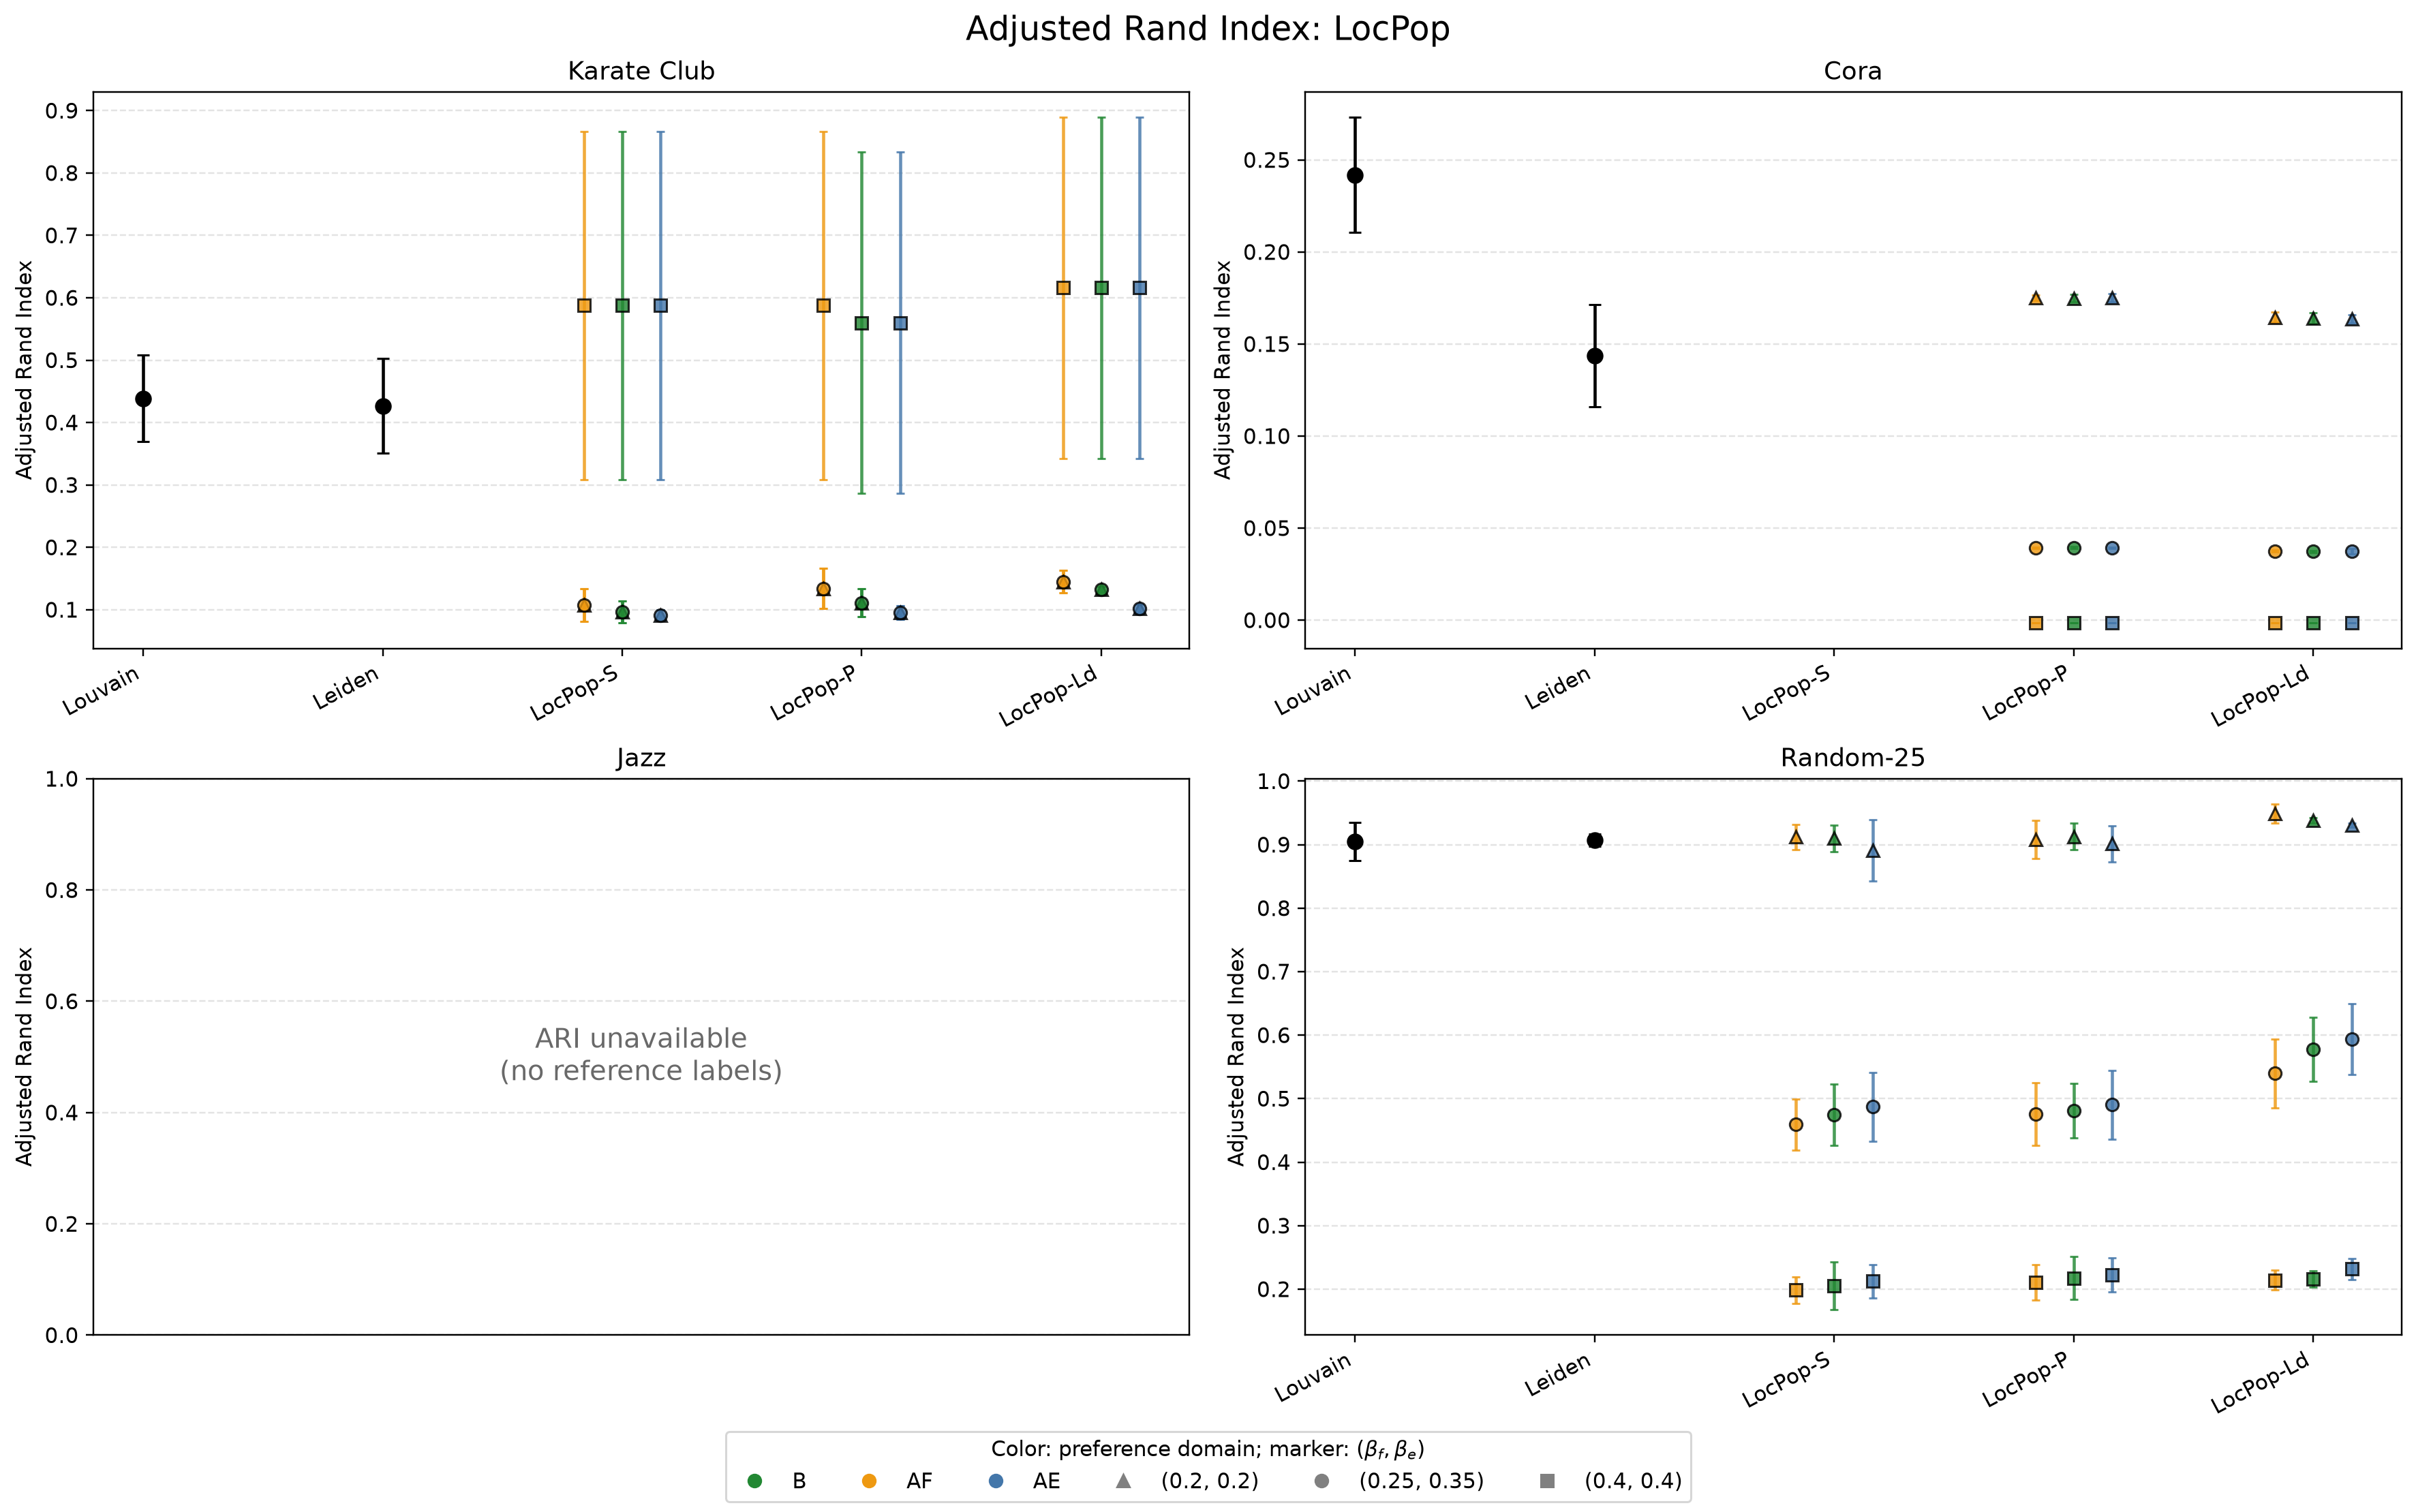
\includegraphics[width=.78\textwidth]{figures/PopularCommunity/summary-Adjusted-Rand-Index.png}
\par\medskip
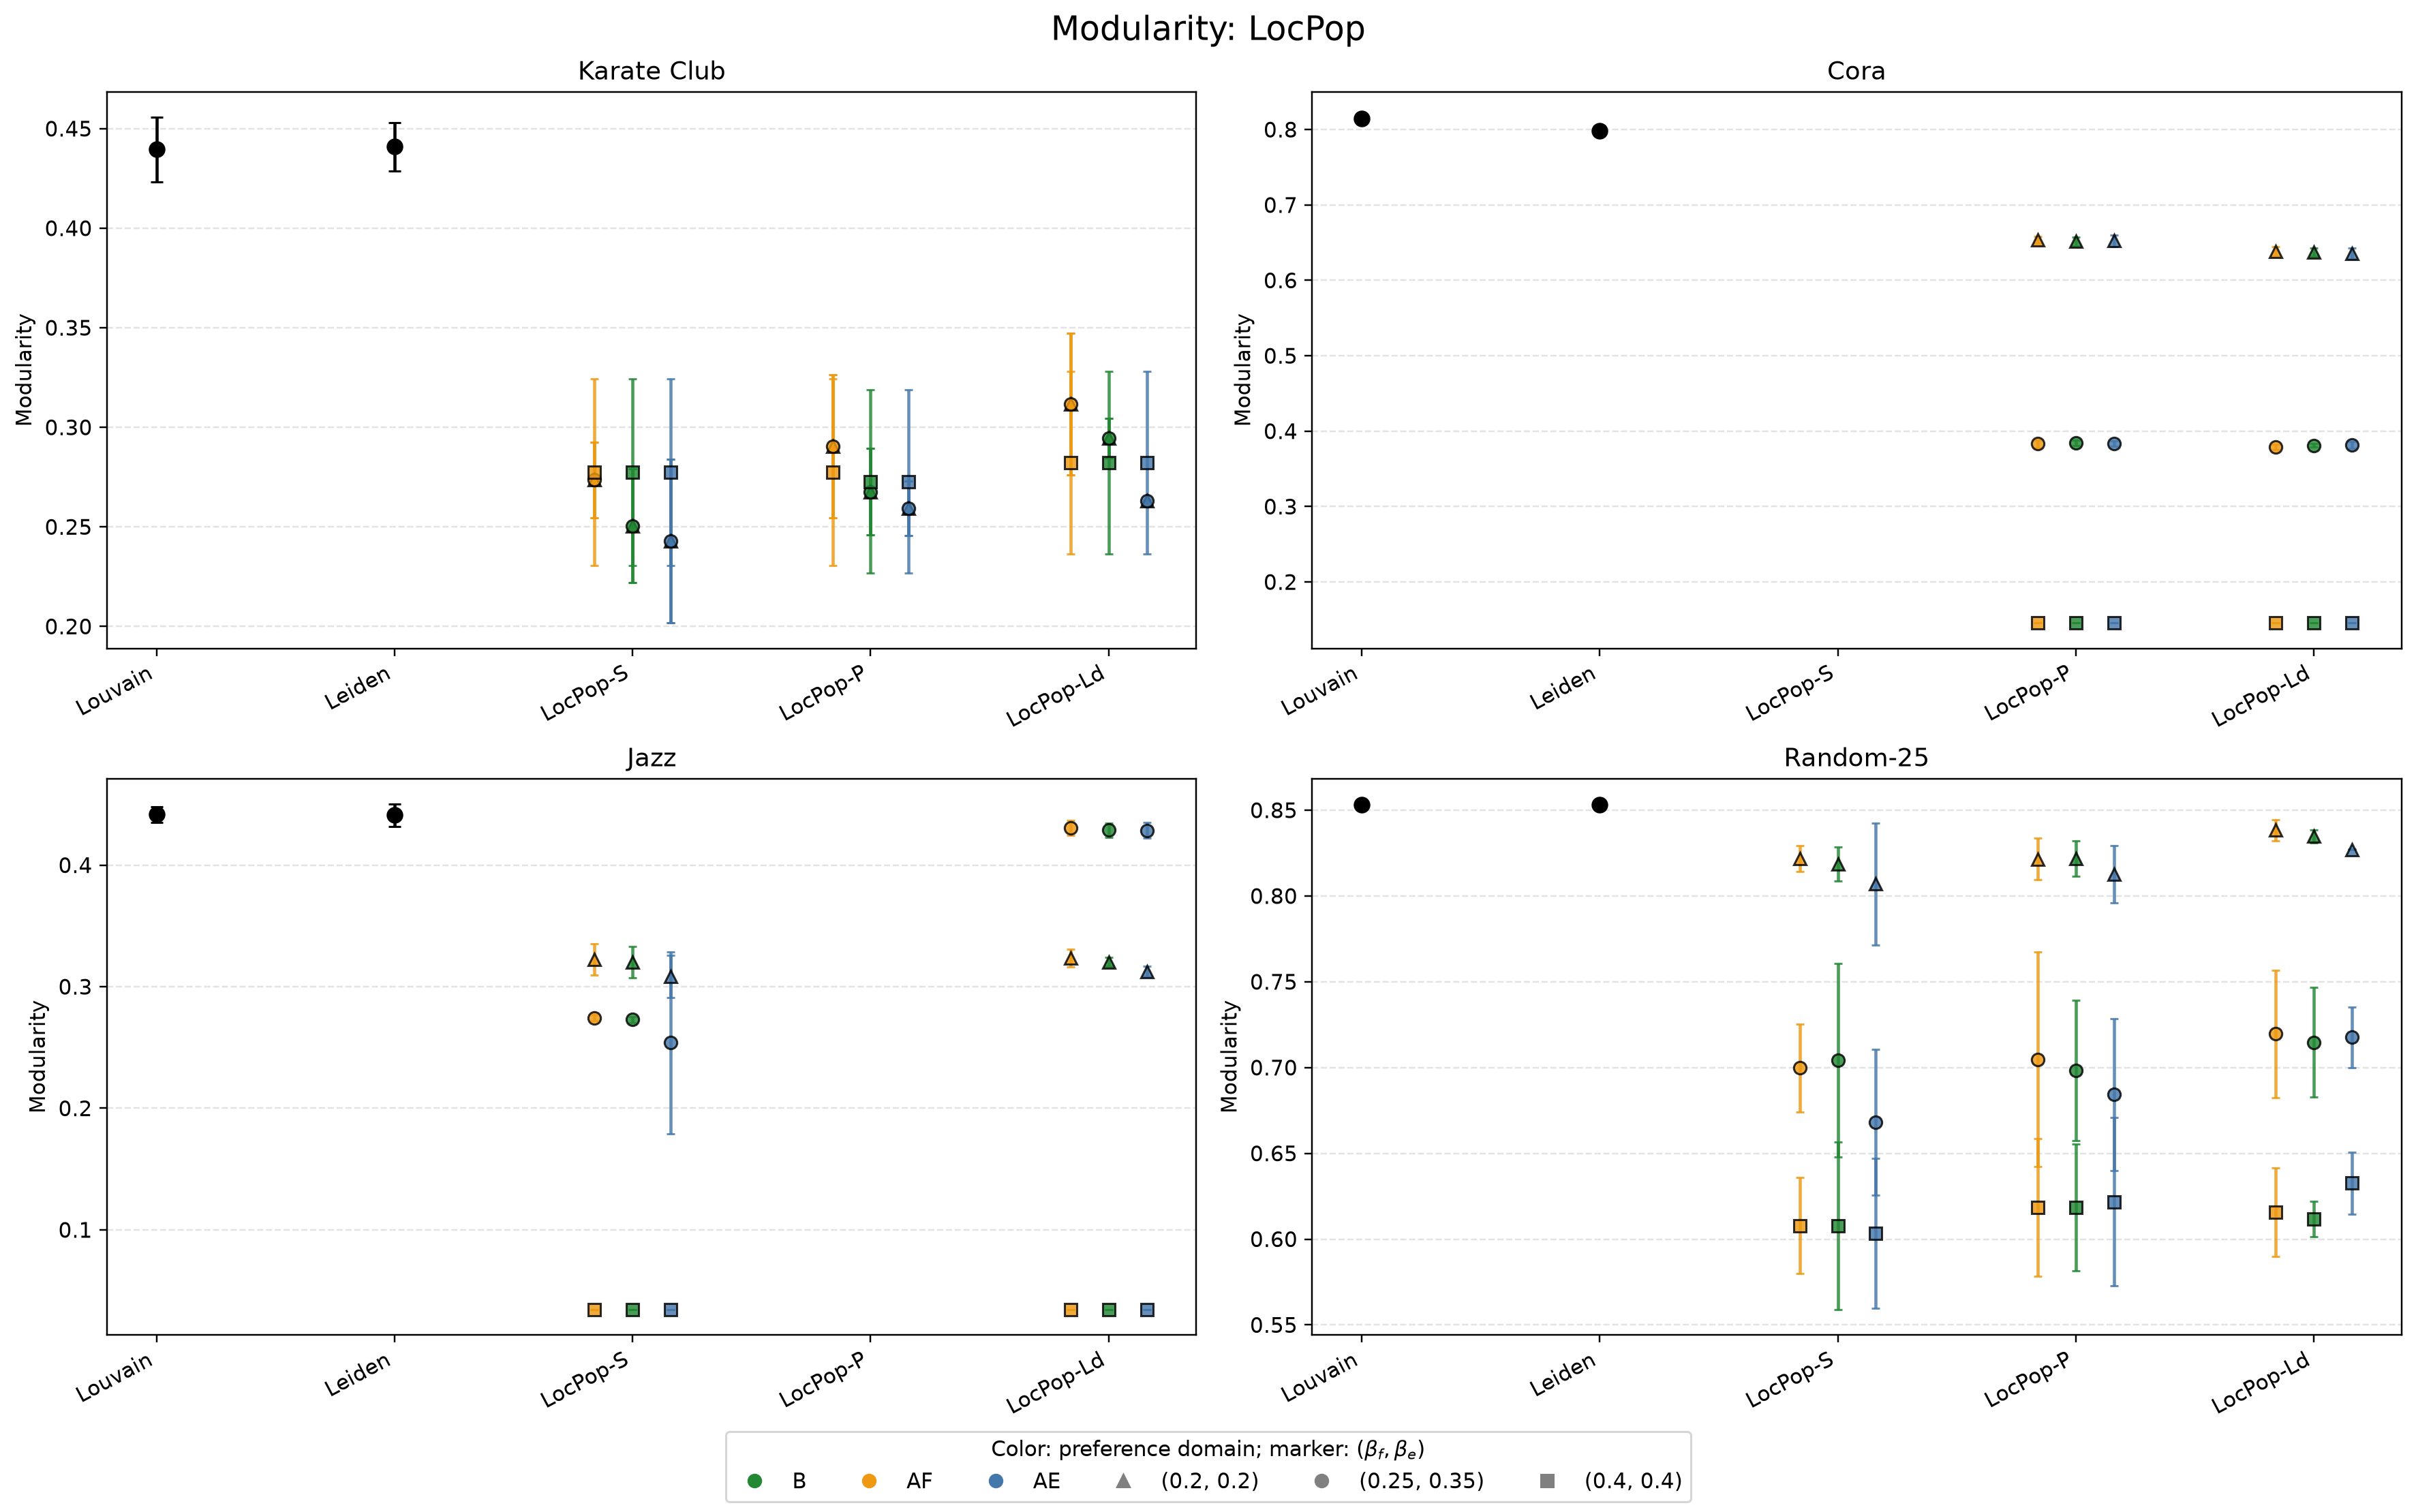
\includegraphics[width=.78\textwidth]{figures/PopularCommunity/summary-Modularity.png}
\caption{\alglocpop\ on the community-detection data sets.  Top: adjusted Rand
index; bottom: modularity.  Each panel contains all available initializations,
preference domains, and threshold pairs.  The legend mapping is described in
Section~\ref{sec:sim-design}.}
\label{fig:sim-community-locpop}
\end{figure}

\begin{figure}[p]
\centering
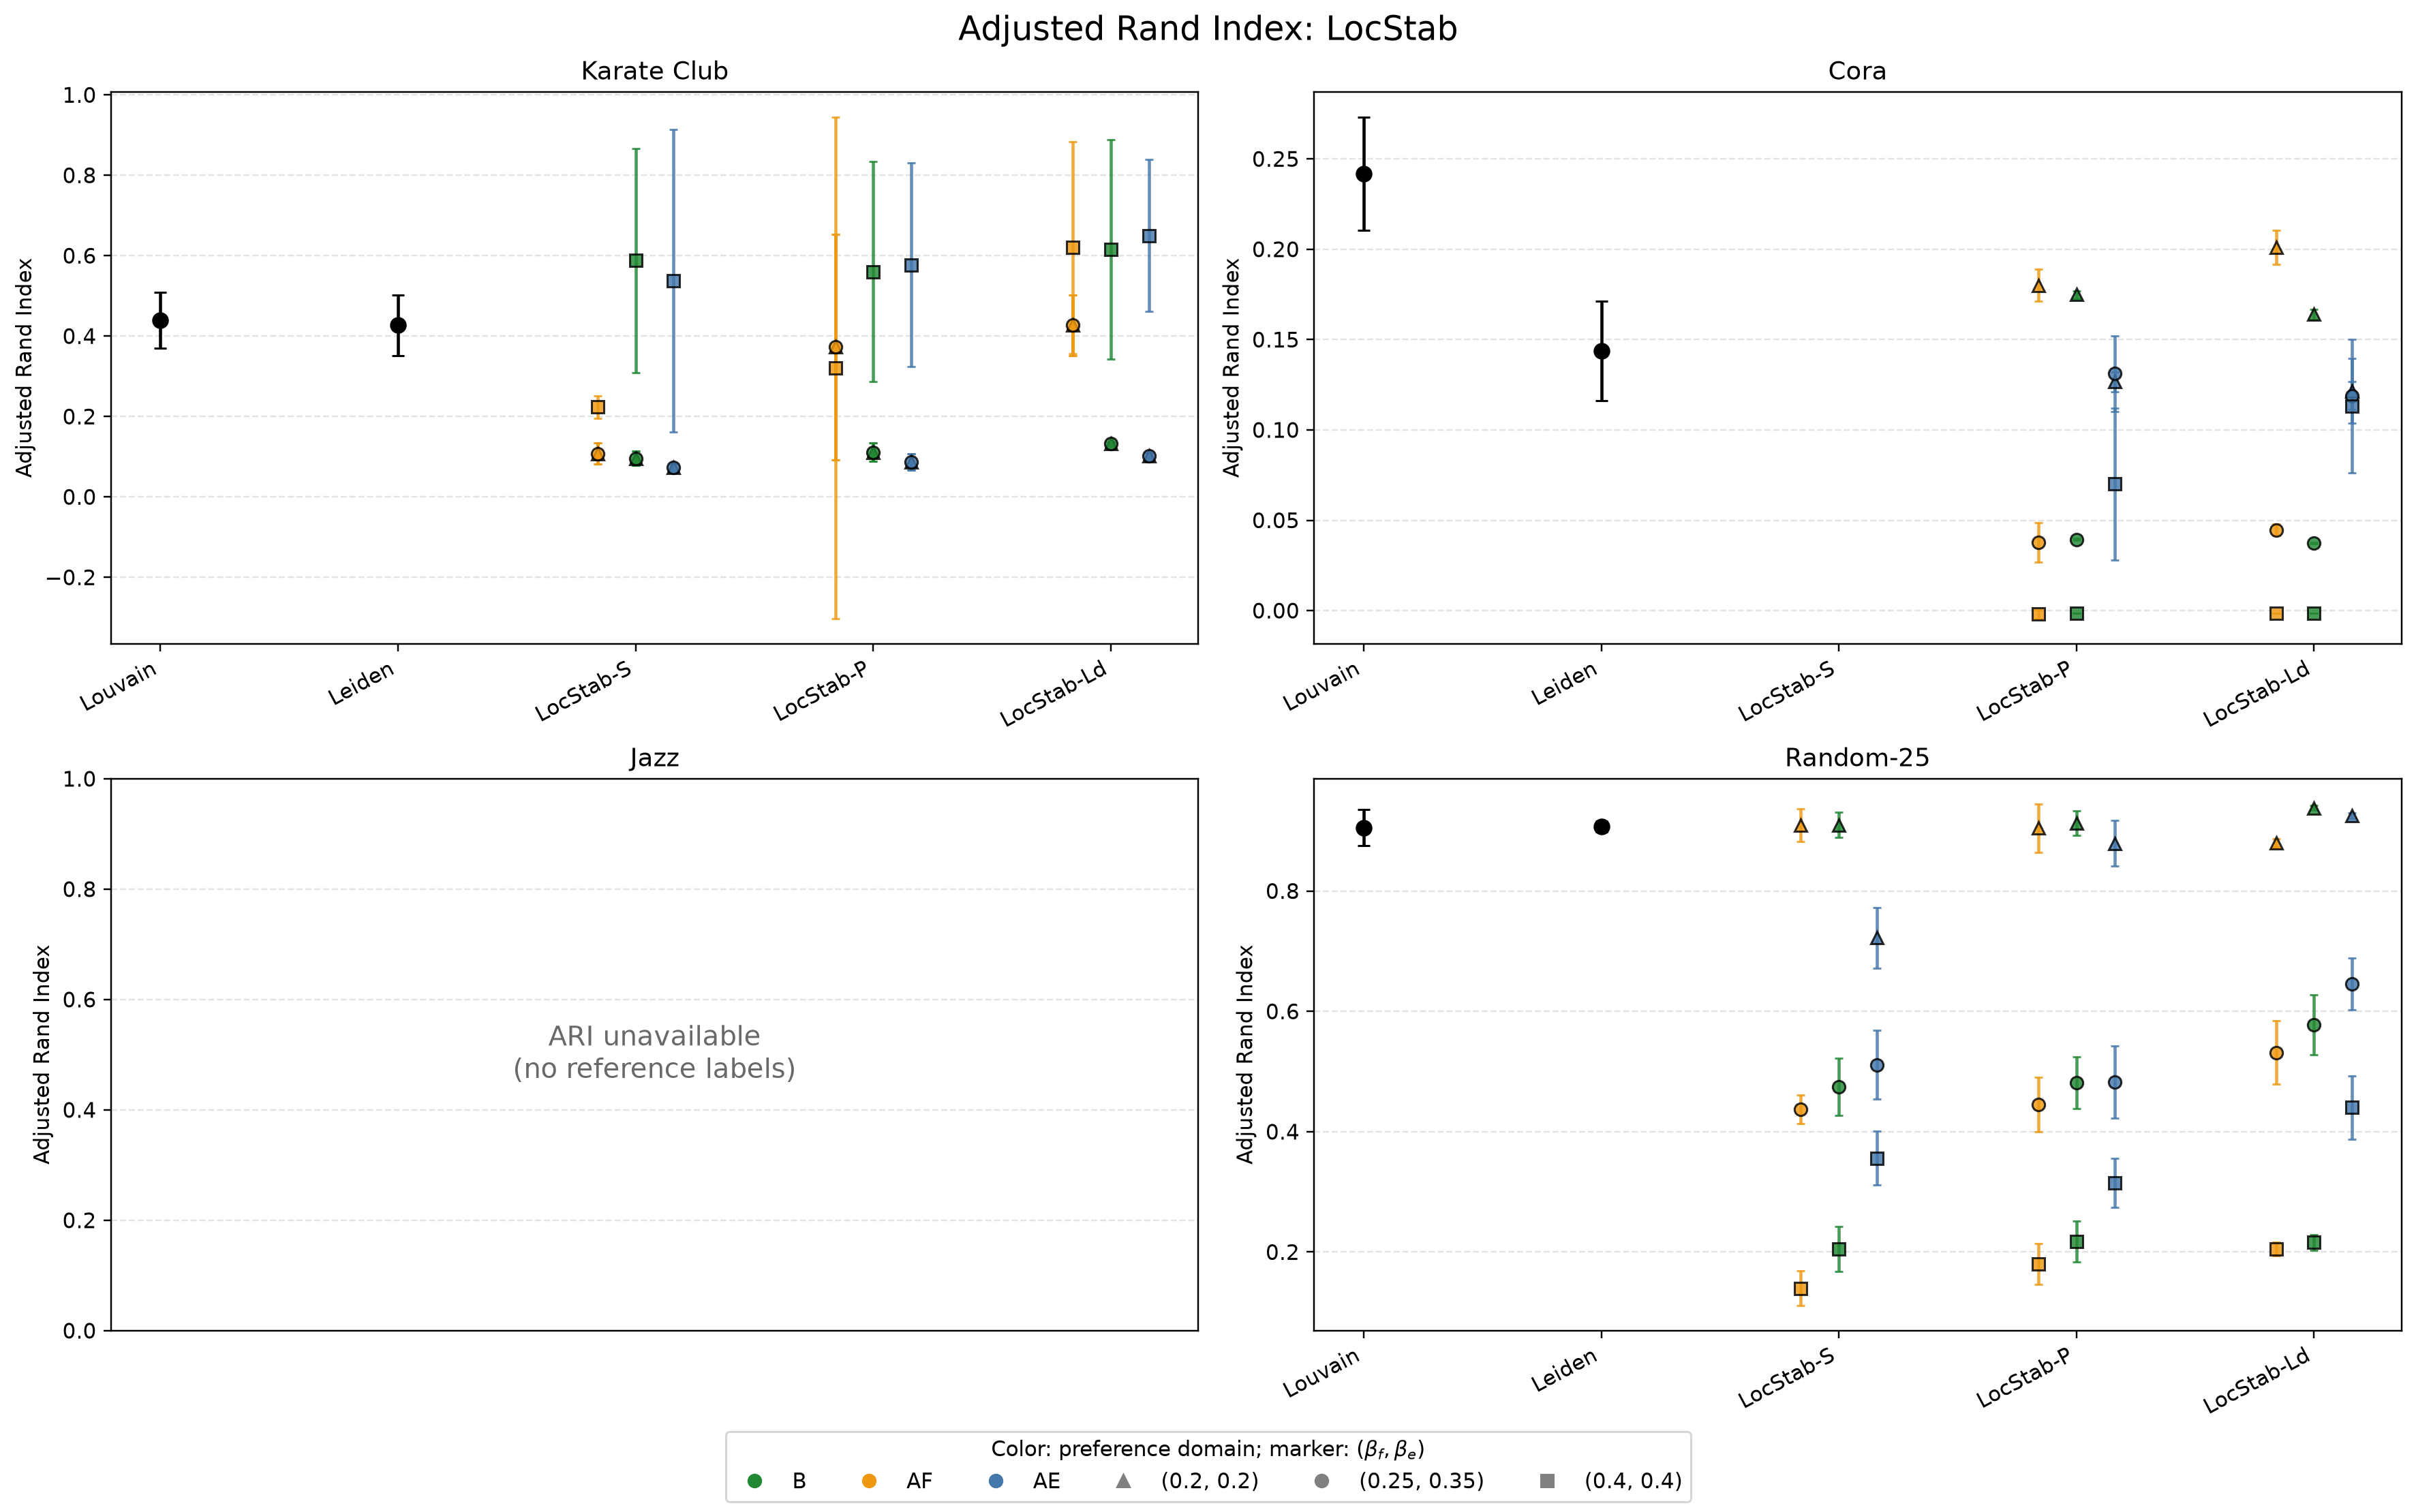
\includegraphics[width=.78\textwidth]{figures/StableCommunity/summary-Adjusted-Rand-Index.png}
\par\medskip
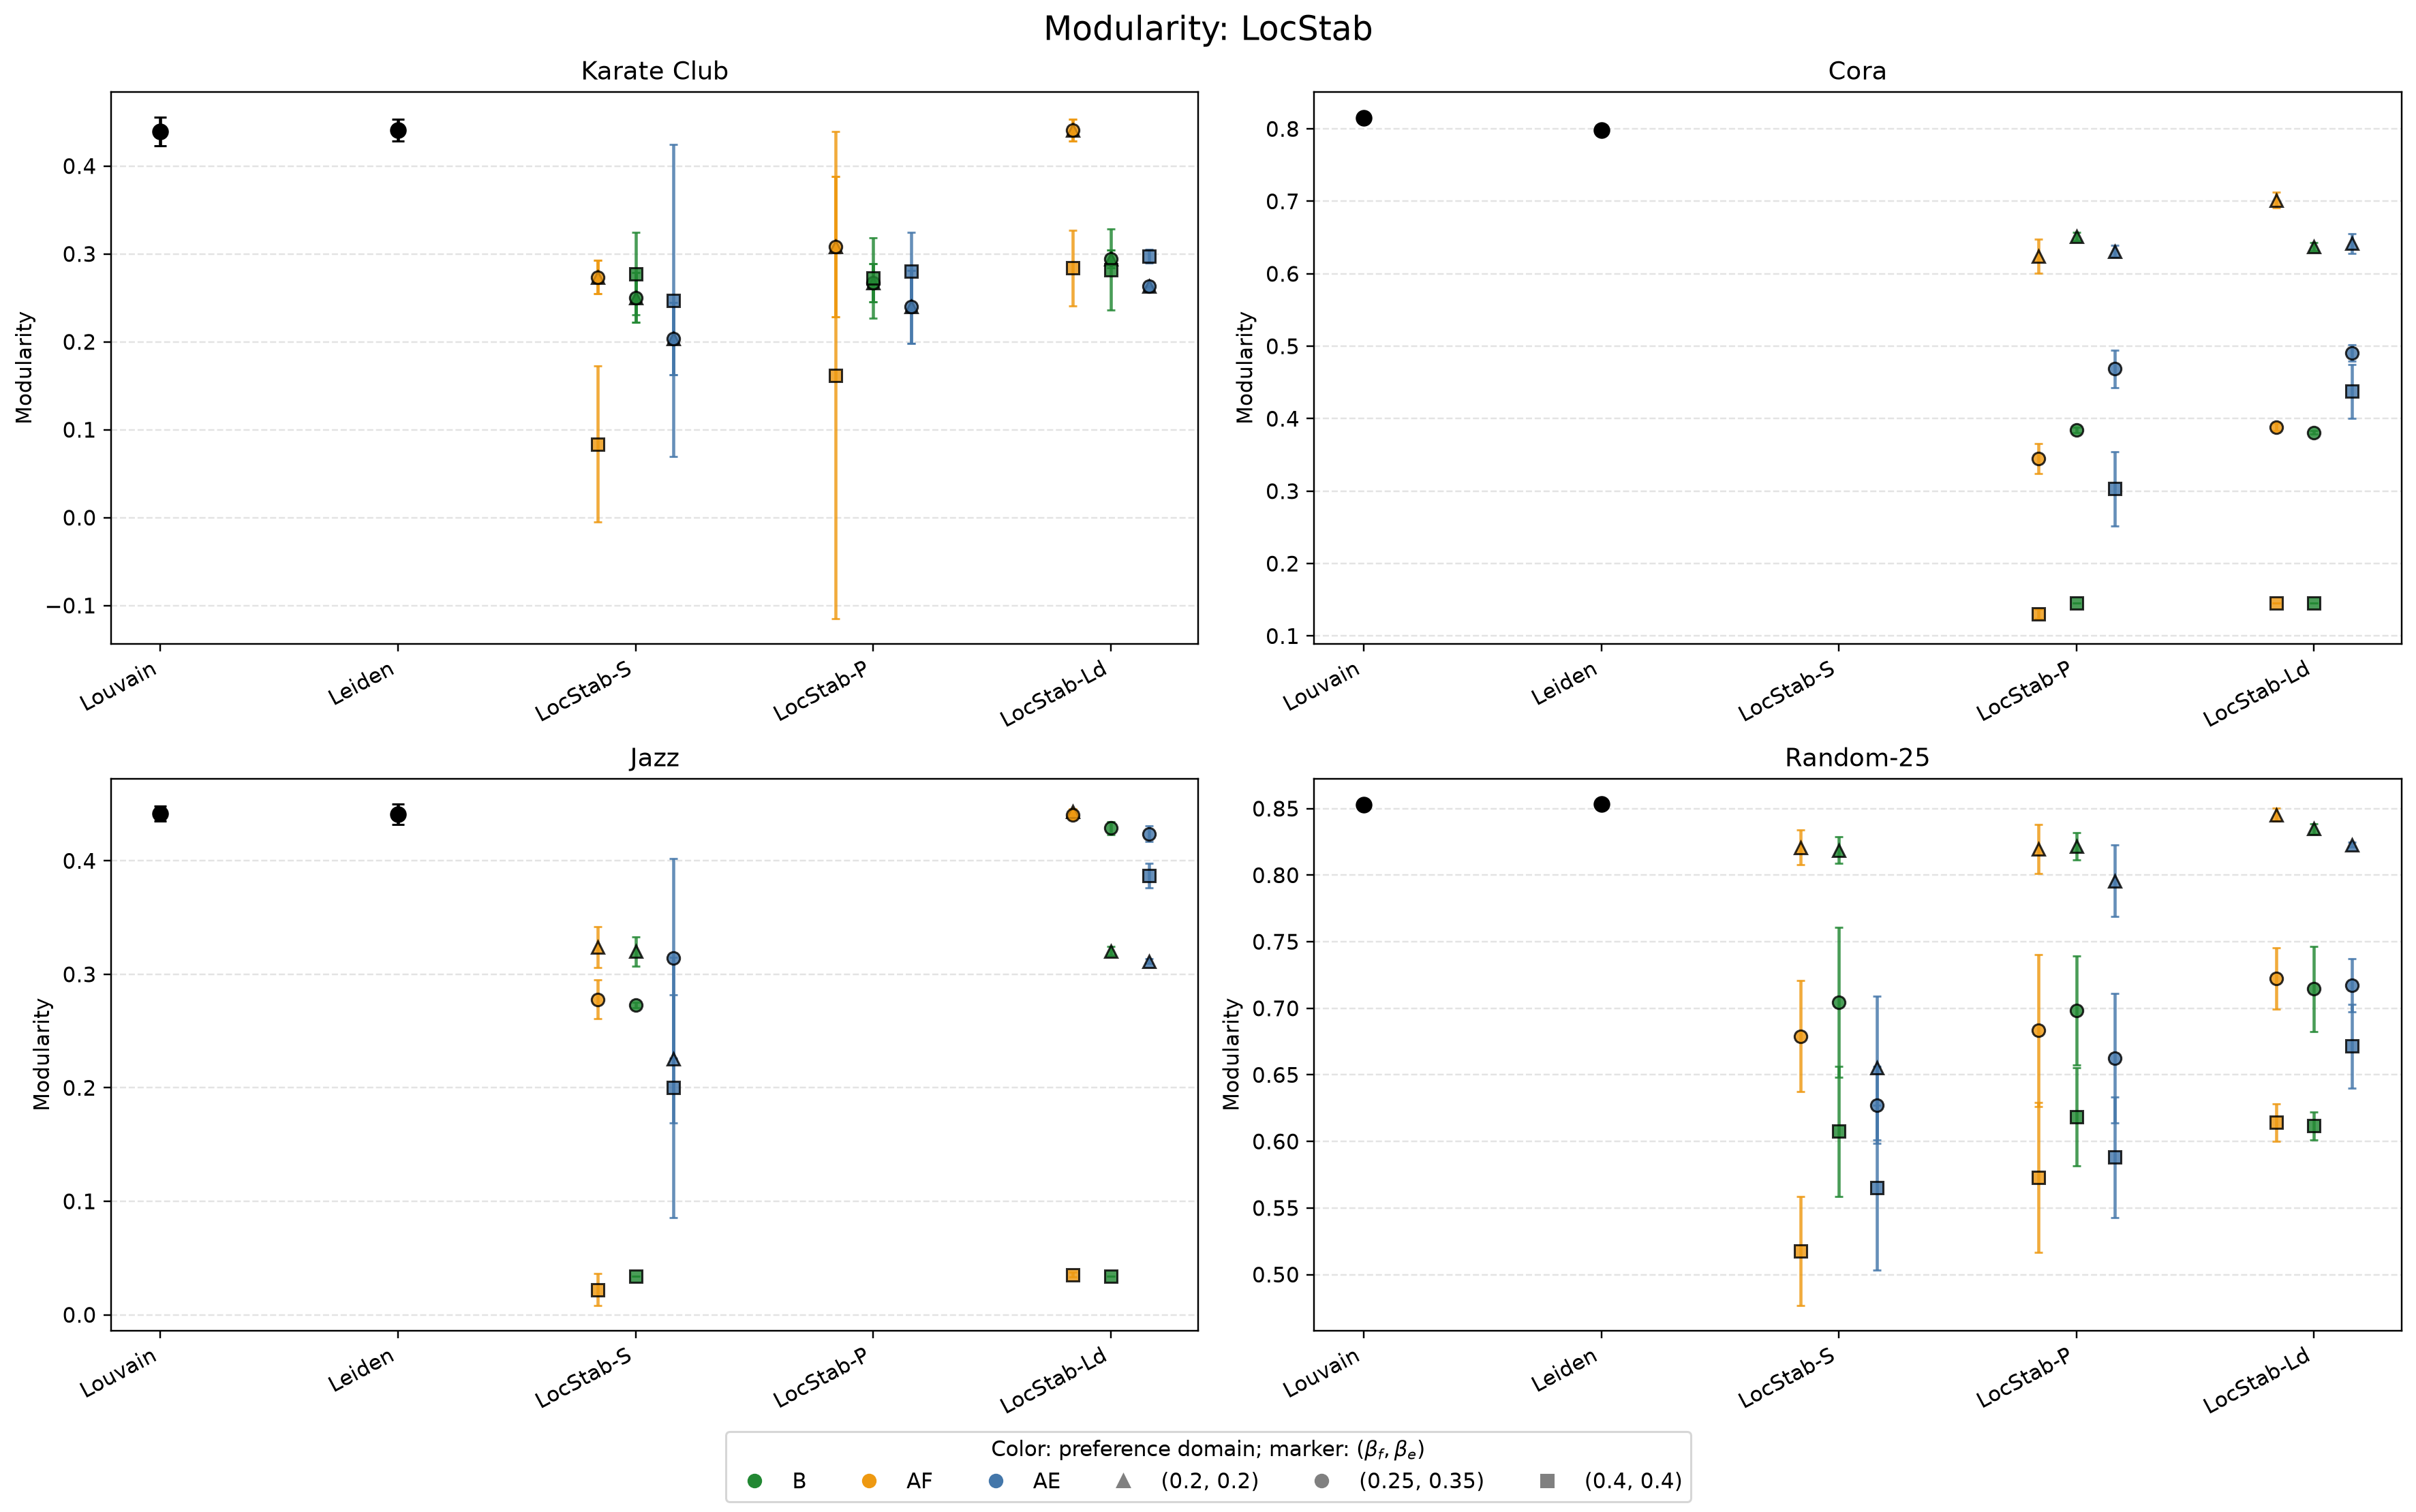
\includegraphics[width=.78\textwidth]{figures/StableCommunity/summary-Modularity.png}
\caption{\alglocstab\ on the community-detection data sets.  Top: adjusted Rand
index; bottom: modularity.  Jazz is annotated as unavailable in the ARI figure
because the data set has no reference partition.}
\label{fig:sim-community-locstab}
\end{figure}

\subsubsection{Vector clustering}
\label{sec:sim-clustering}

The strongest clustering result is on 3 Circles.  The best mean ARI is
\(0.467\) for \alglocpop\ and \(0.468\) for \alglocstab, compared with
\(0.444\) for \(k\)-means and \(0.187\) for DBSCAN.  The heuristics also reach
silhouette \(0.479\), compared with \(0.410\) for \(k\)-means.  The
ARI-optimal \alglocpop\ configuration (a \(k\)-means warm start, B preferences,
and threshold \((0.40,0.40)\)) achieves both improvements simultaneously.
This is evidence that a locally justified sequence of switches can repair a
useful but imperfect baseline partition.

On Iris, \alglocstab\ gives a smaller but consistent improvement: its best ARI
is \(0.627\), compared with \(0.617\) for \(k\)-means, and its best silhouette
is \(0.495\), compared with \(0.460\).  \alglocpop\ does not match these values.
On Cancer, neither heuristic surpasses the \(k\)-means ARI of \(0.667\);
\alglocstab\ comes closest at \(0.634\).  Although \alglocstab\ can obtain a
substantially larger silhouette (\(0.462\) versus \(0.345\)), that
silhouette-optimal configuration has ARI only \(0.063\).  The analogous
\alglocpop\ configuration has silhouette \(0.360\) and ARI \(0.059\).  This
sharp disagreement cautions against interpreting geometric separation as
recovery of the diagnostic labels.

Moons exhibits the converse metric mismatch.  DBSCAN nearly perfectly recovers
the two non-convex classes (ARI \(0.993\)) but has silhouette \(0.018\), while
\(k\)-means has silhouette \(0.488\) and ARI \(0.479\).  The best
\alglocpop\ ARI is only \(0.327\).  \alglocstab\ can retain the DBSCAN
partition unchanged under AF preferences and threshold \((0.20,0.20)\), hence
matching its ARI, while other settings trade away label recovery for a higher
silhouette.  The zero-switch result is informative: the individual-rationality
filter in \alglocstab\ can protect a strong warm start that the purely
vote-driven rule would modify.

Threshold sensitivity again dominates any simple algorithm ranking.  For
Cancer, increasing the threshold raises the mean silhouette but reduces mean
ARI; for Iris, the high threshold improves both measures; for Moons, the
intermediate threshold is strongest on average; and for 3 Circles, the best
choice depends on the metric and heuristic.  These interactions rule out the
claim that either a sparse or dense relation is uniformly preferable.

\begin{figure}[p]
\centering
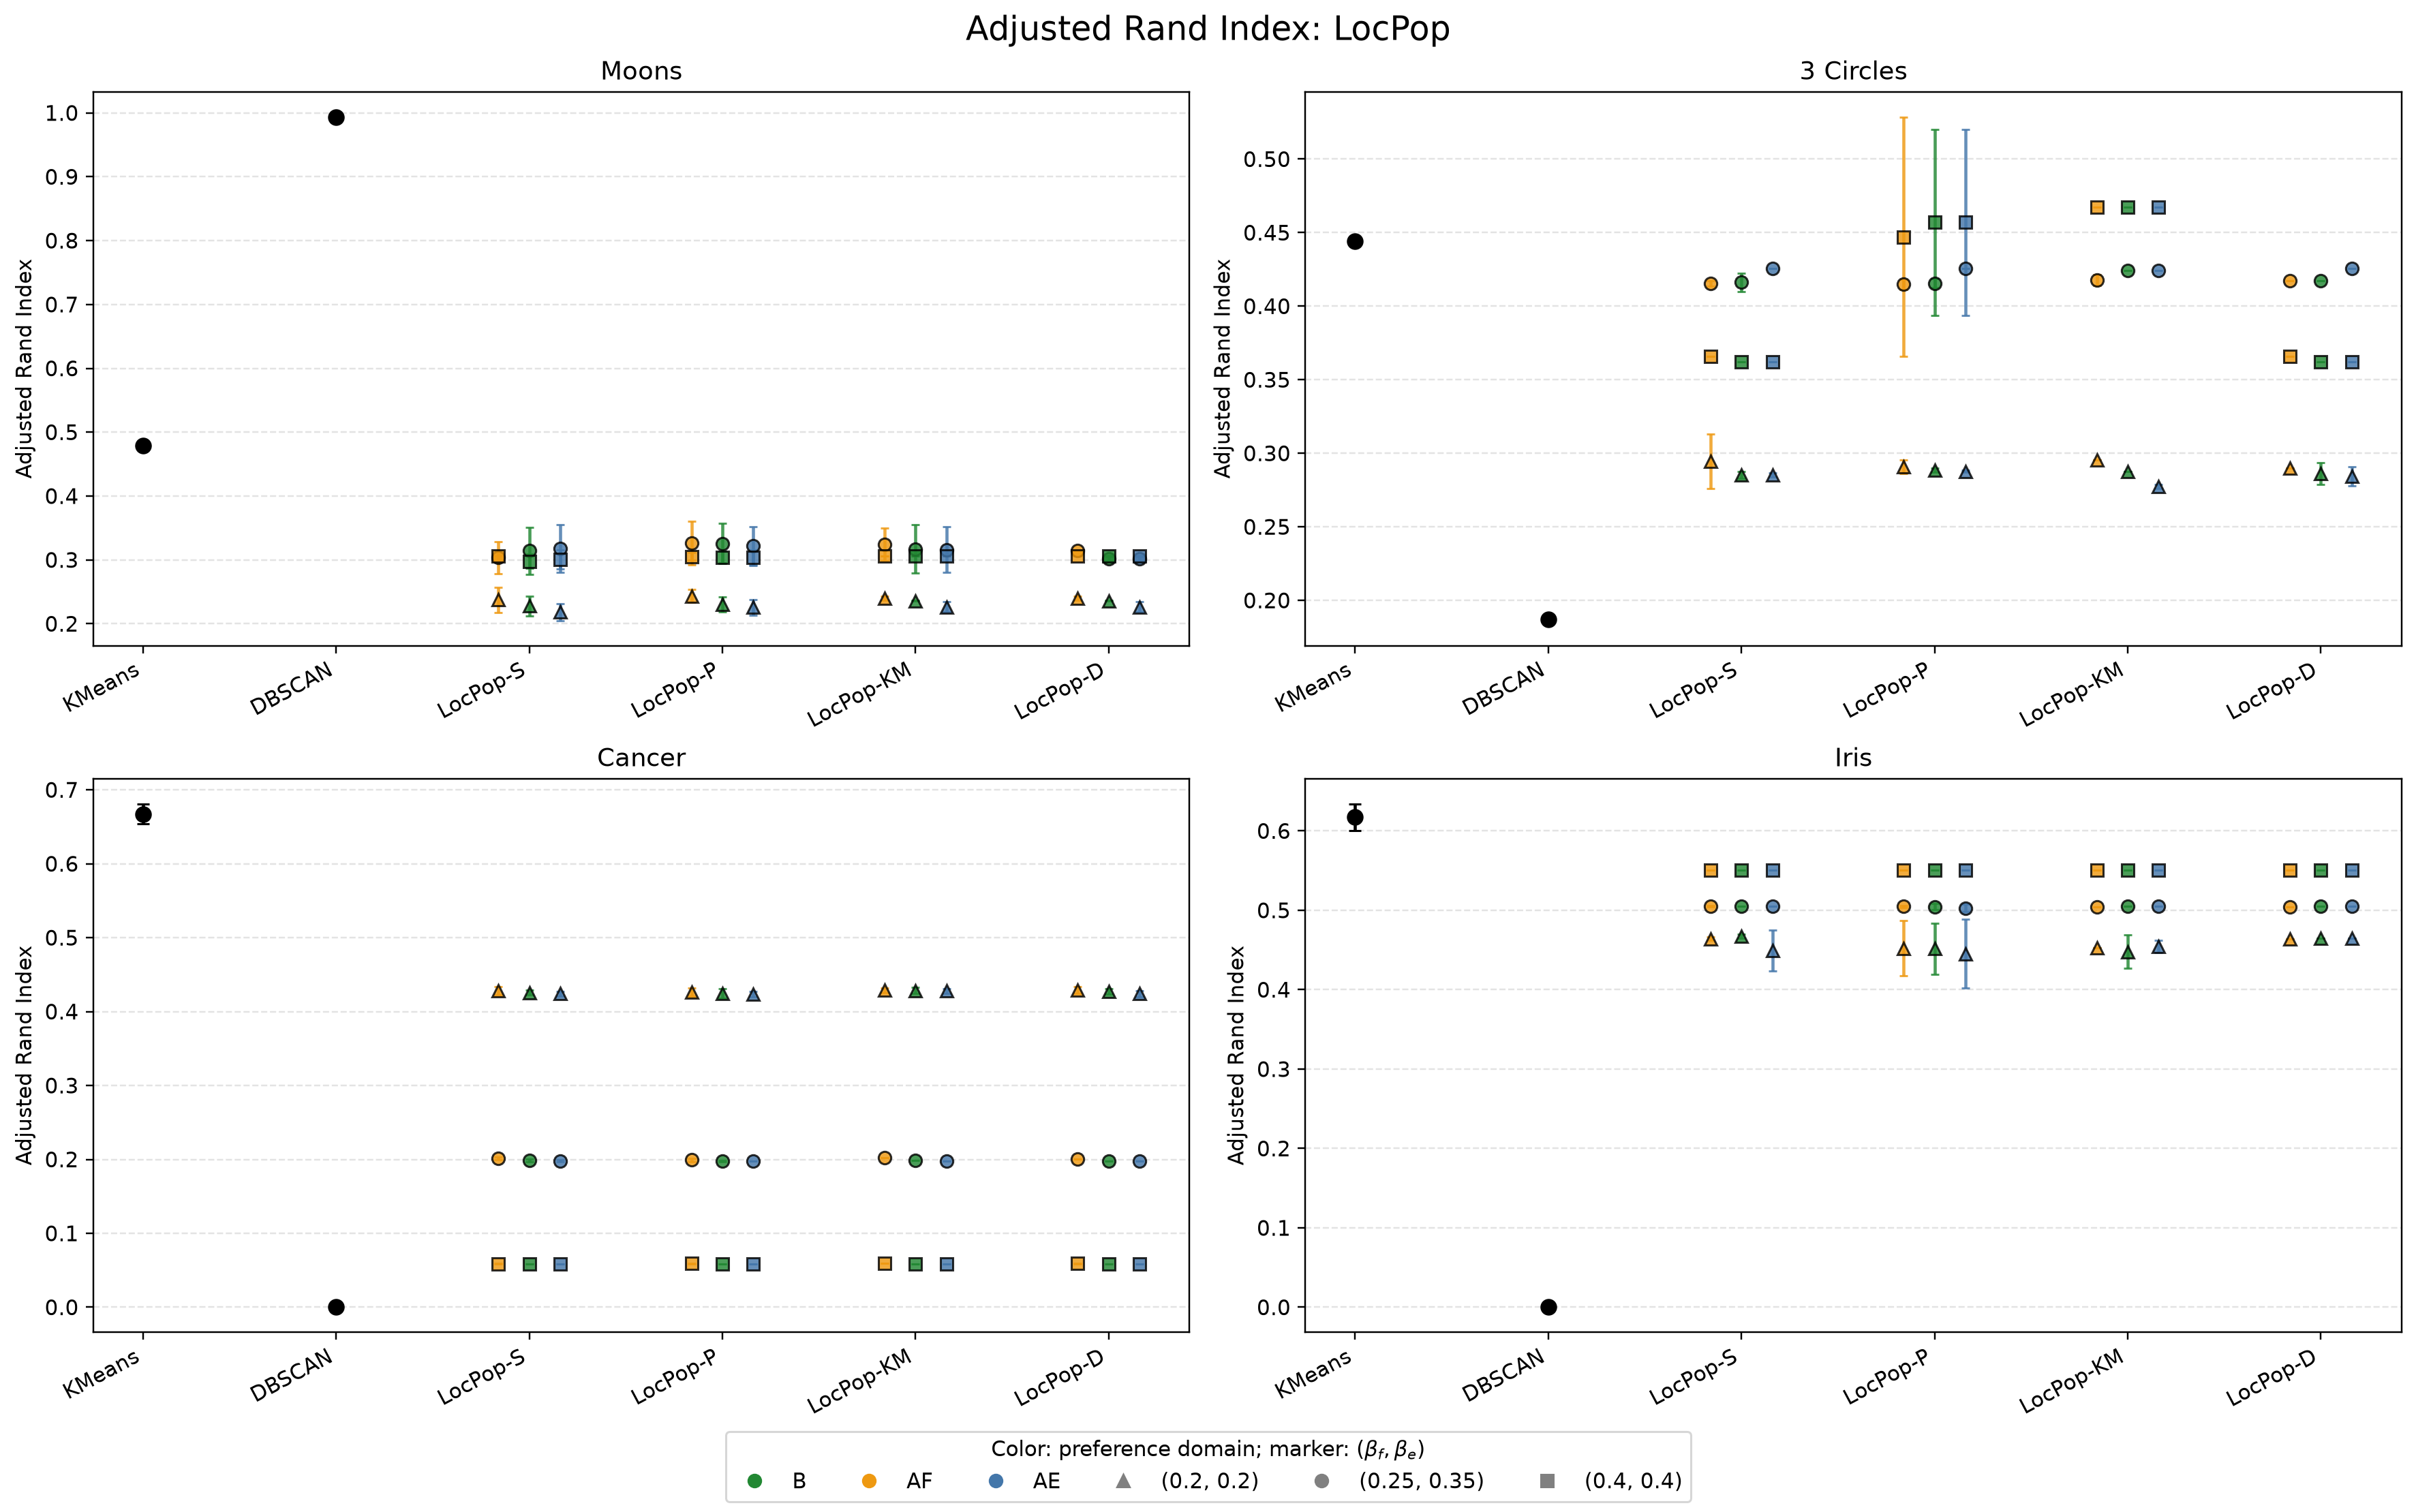
\includegraphics[width=.78\textwidth]{figures/PopularClustering/summary-Adjusted-Rand-Index.png}
\par\medskip
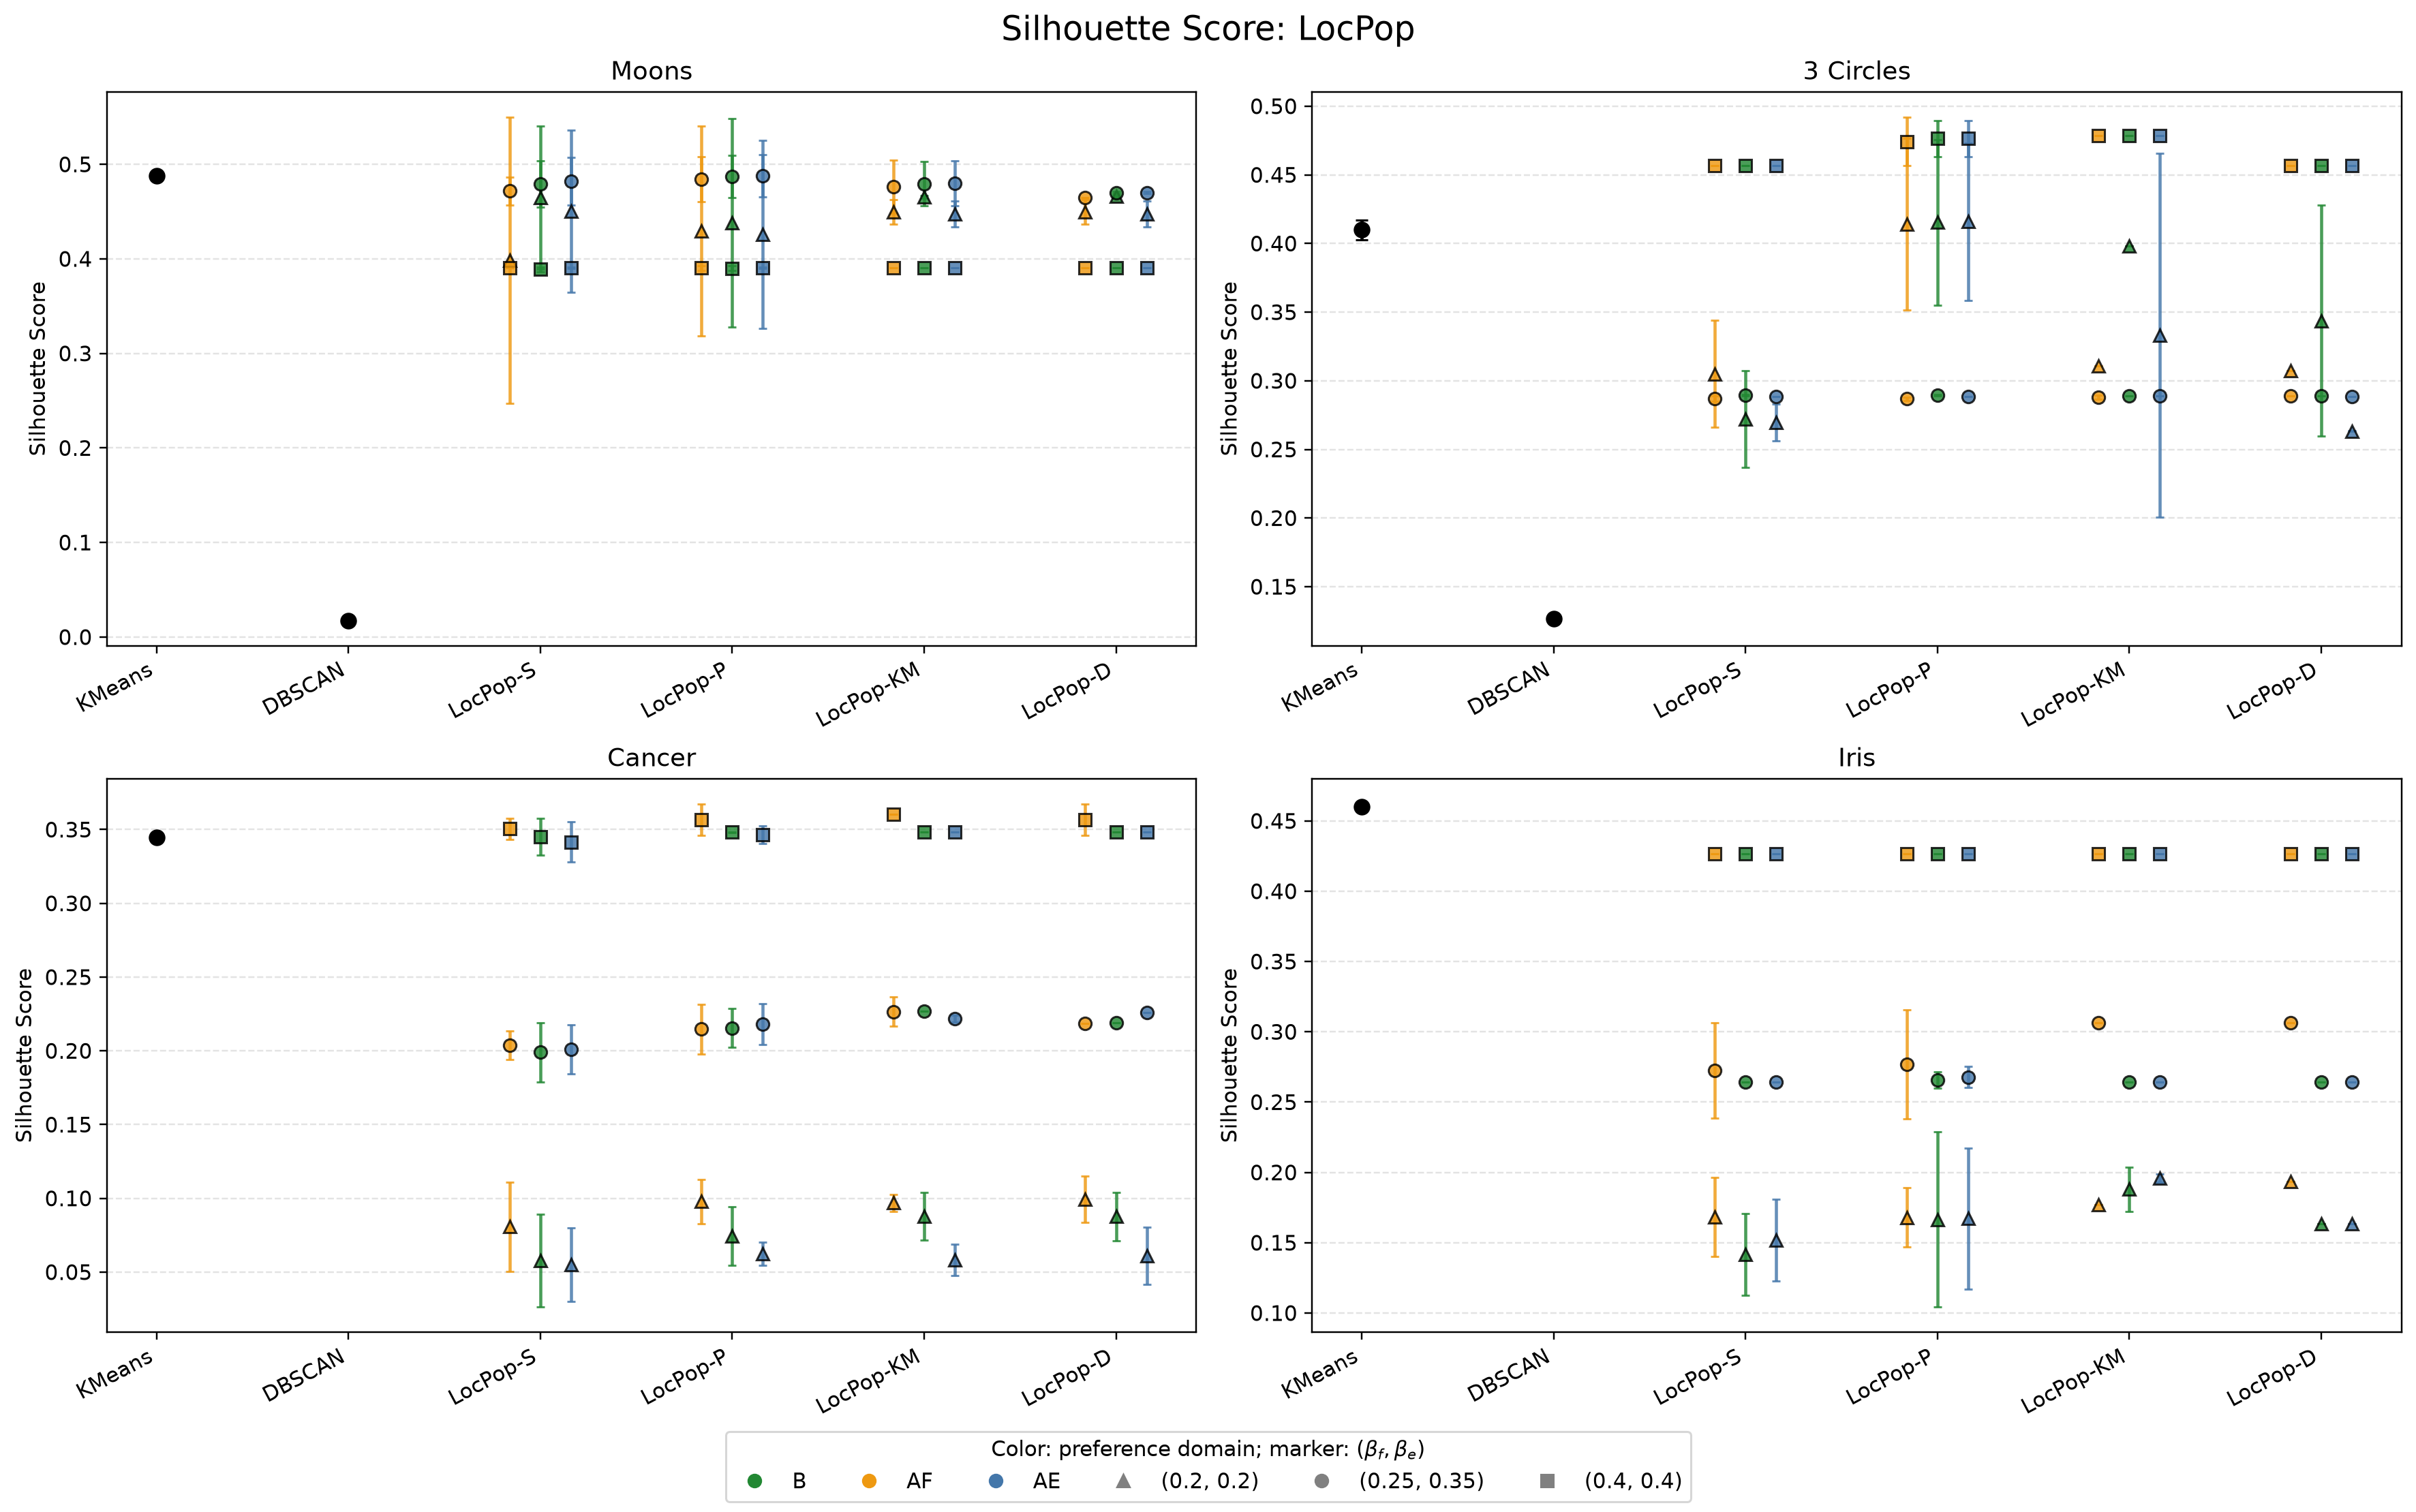
\includegraphics[width=.78\textwidth]{figures/PopularClustering/summary-Silhouette-Score.png}
\caption{\alglocpop\ on the vector-clustering data sets.  Top: adjusted Rand
index; bottom: silhouette score.  Missing silhouette values correspond to
partitions for which the score is undefined.}
\label{fig:sim-clustering-locpop}
\end{figure}

\begin{figure}[p]
\centering
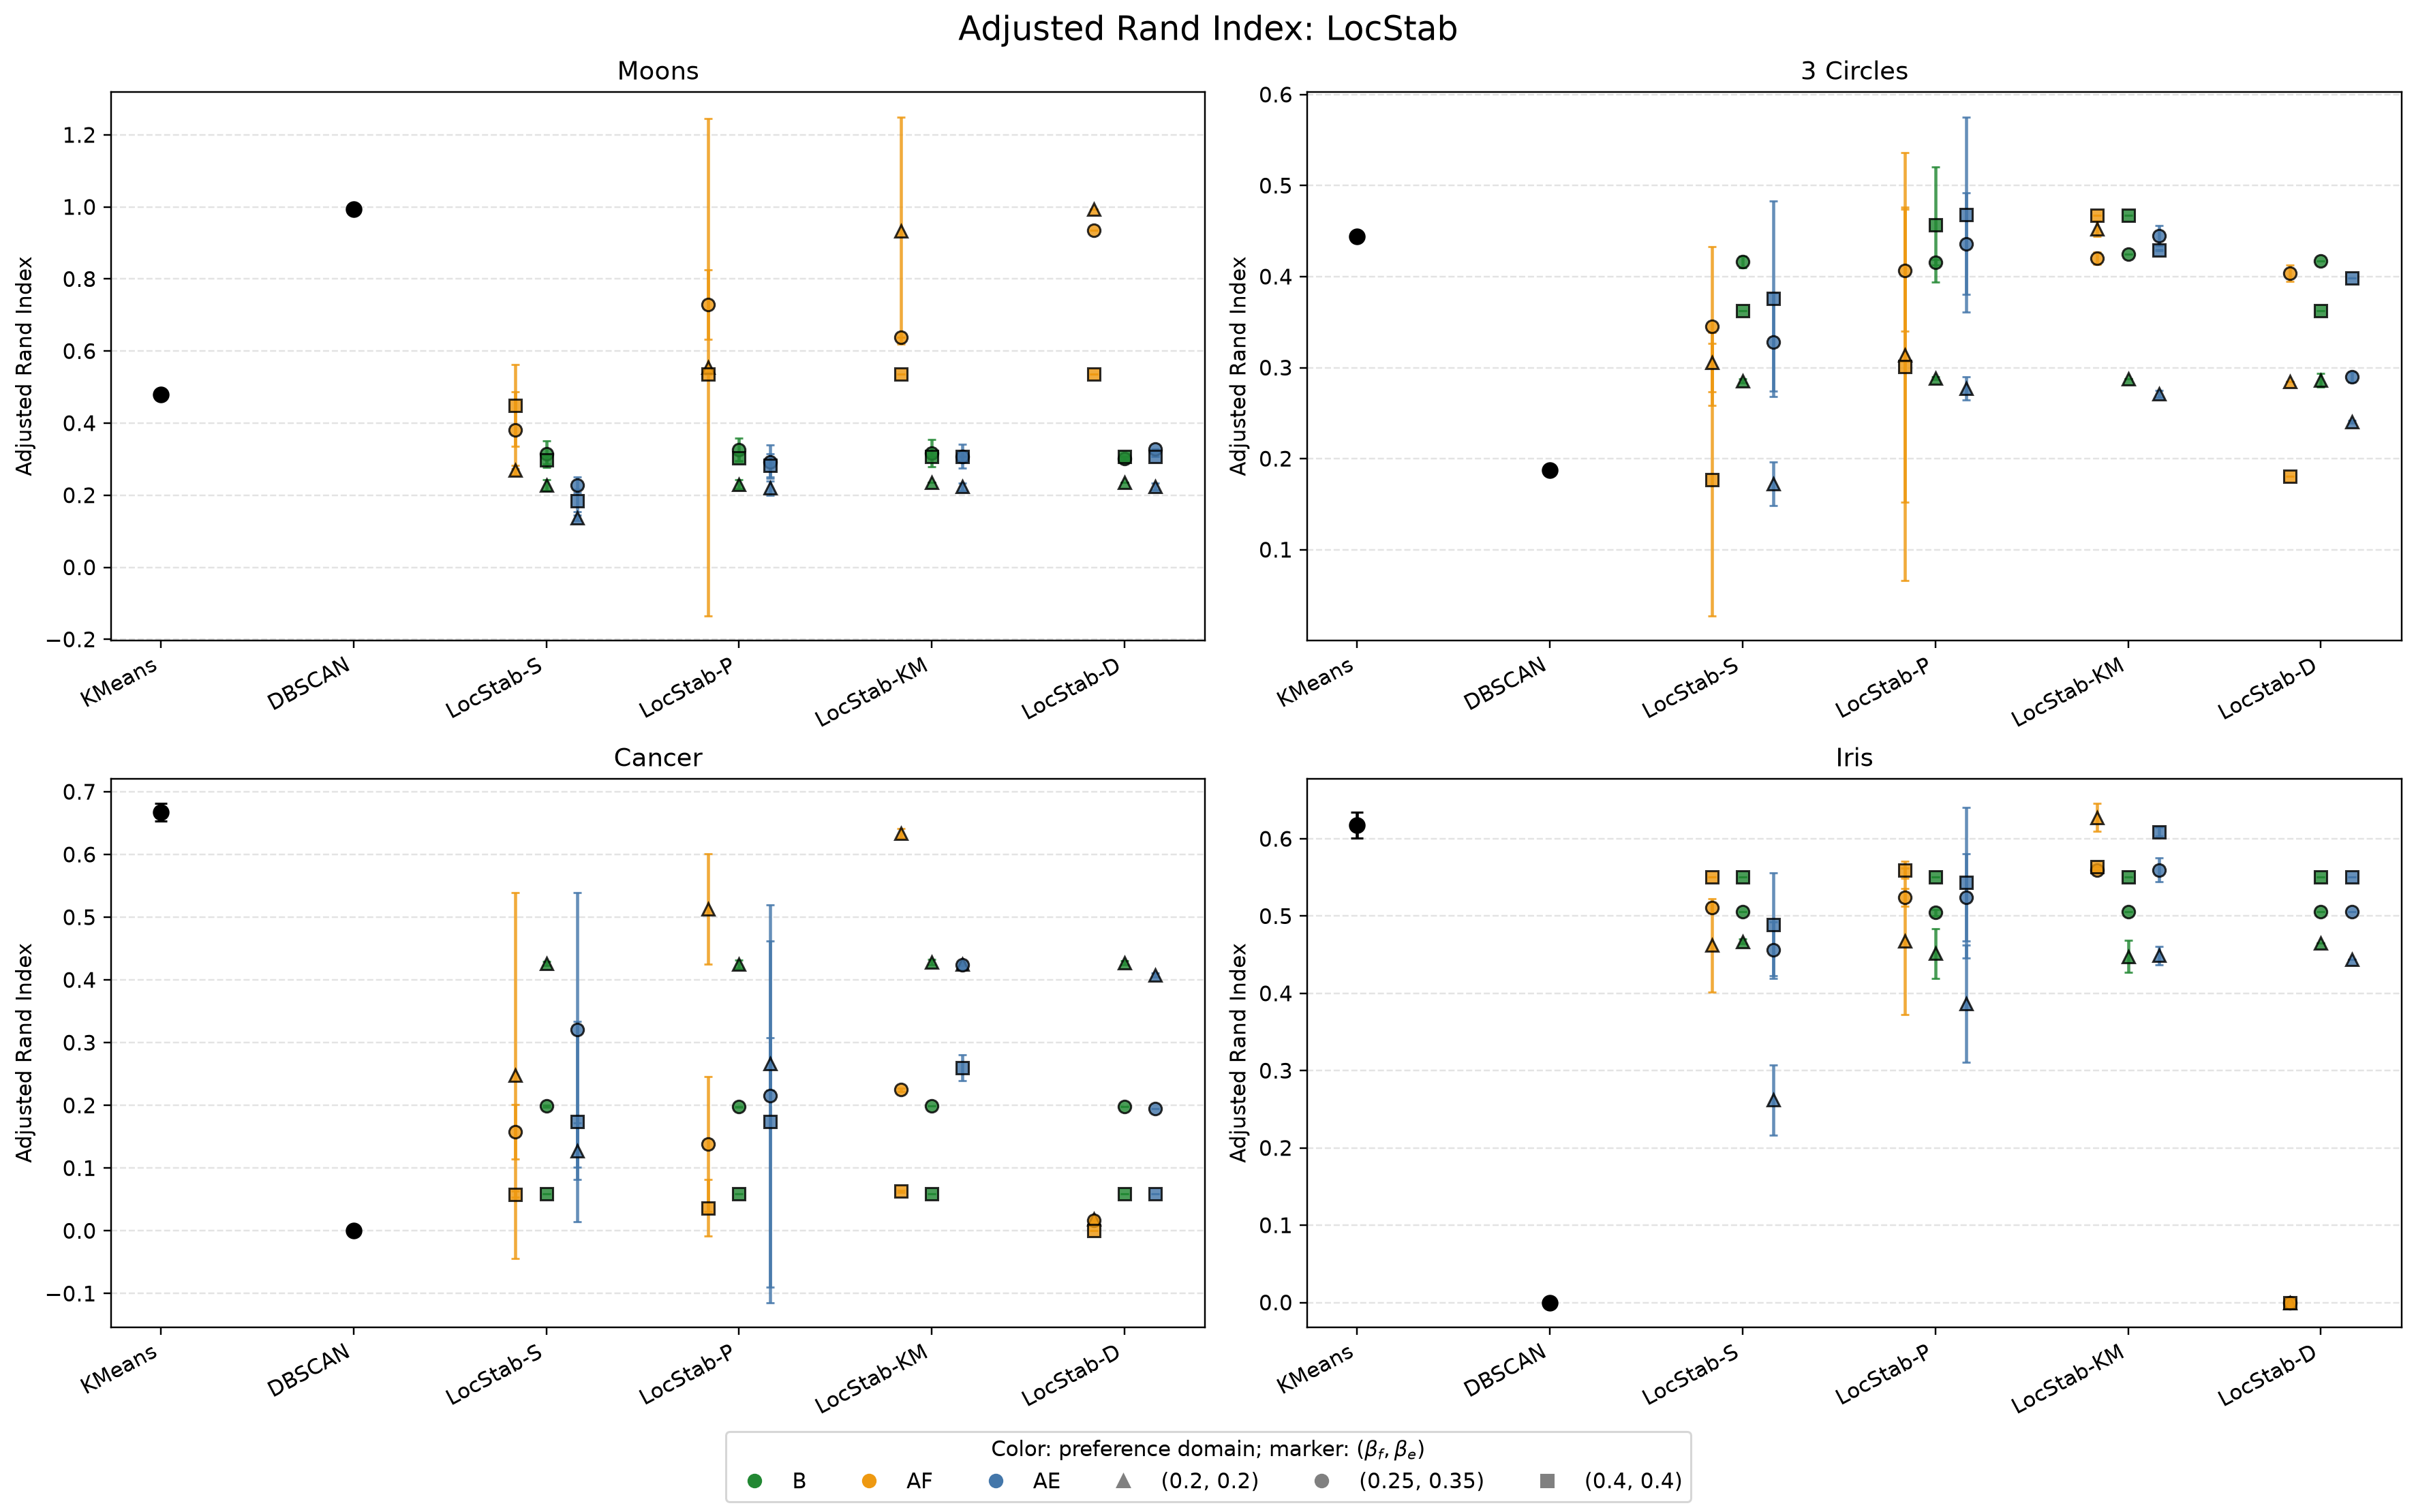
\includegraphics[width=.78\textwidth]{figures/StableClustering/summary-Adjusted-Rand-Index.png}
\par\medskip
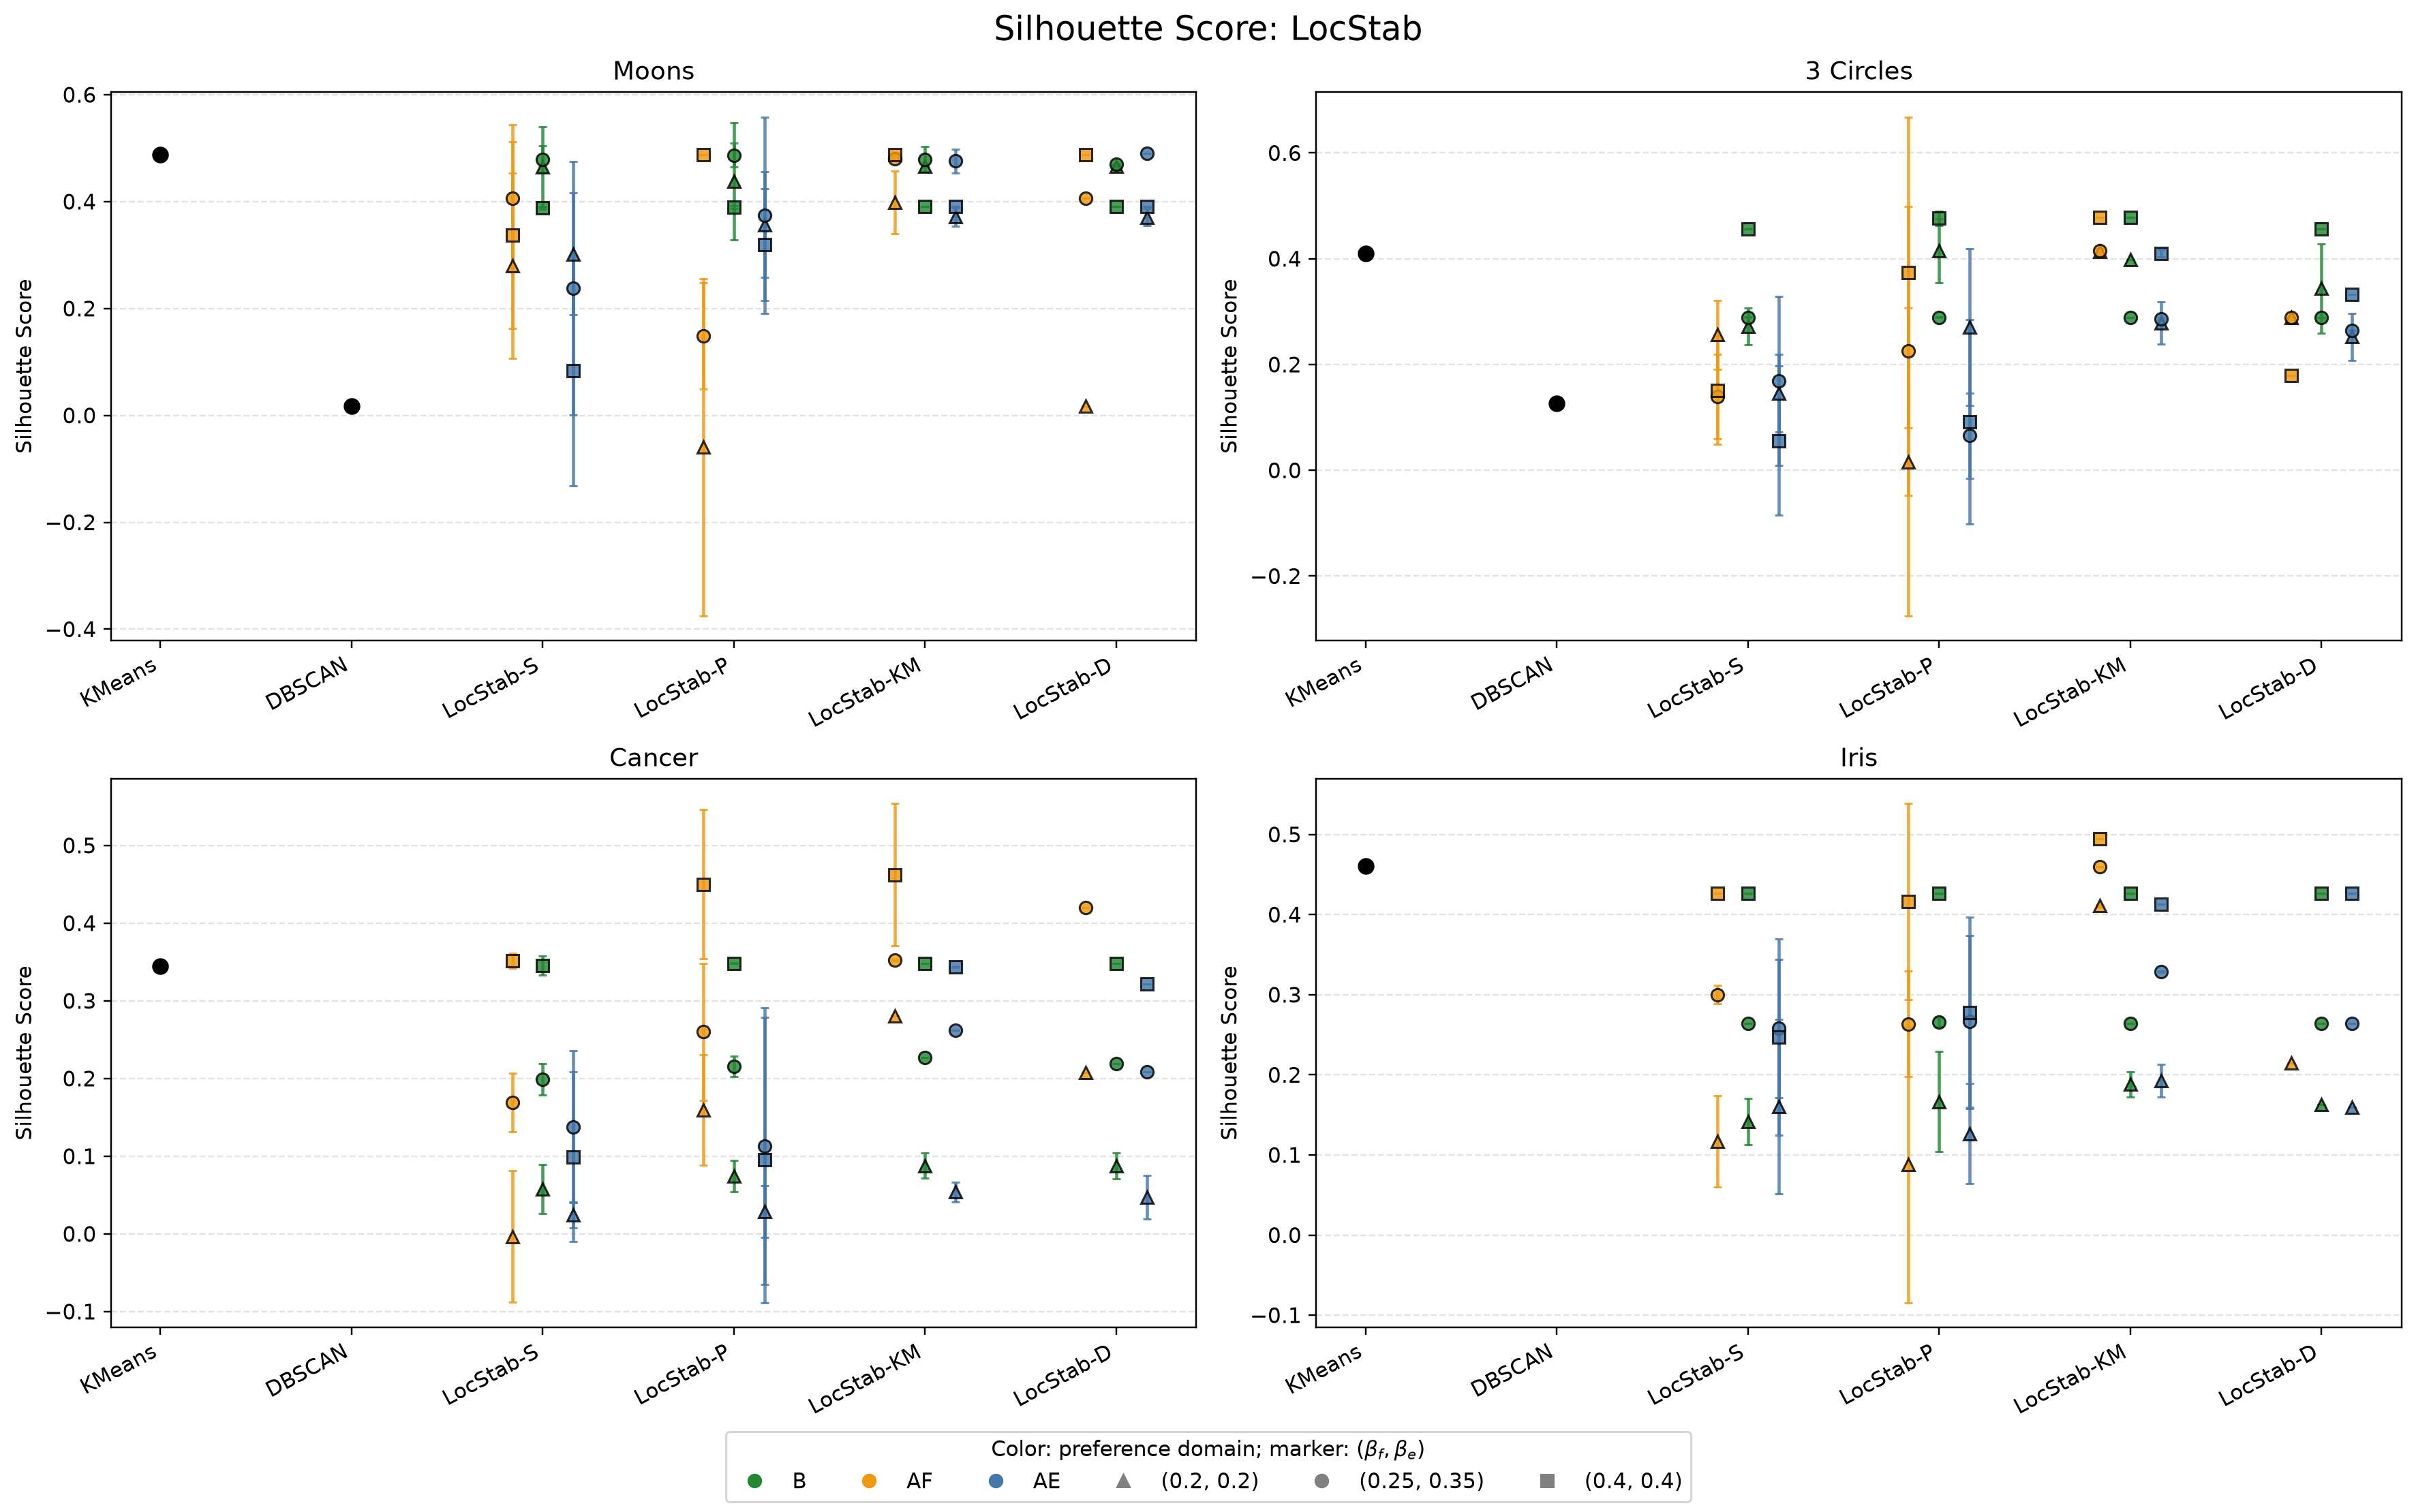
\includegraphics[width=.78\textwidth]{figures/StableClustering/summary-Silhouette-Score.png}
\caption{\alglocstab\ on the vector-clustering data sets.  Top: adjusted Rand
index; bottom: silhouette score.}
\label{fig:sim-clustering-locstab}
\end{figure}

\subsubsection{Preference domains, initialization, and convergence}
\label{sec:sim-sensitivity}

The preference domain has markedly different effects on the two heuristics.
For \alglocpop, the average max--min spread across B, AF, and AE within a fixed
data set/initialization/threshold cell is \(0.006\) ARI for clustering and
\(0.017\) ARI for community detection.  For \alglocstab, the corresponding
spreads are \(0.215\) and \(0.147\).  The same pattern holds for the internal
measures.  The additional individual-improvement condition therefore makes
\alglocstab\ substantially more sensitive to how agents trade friends against
enemies.  No domain is uniformly best: several maxima in
Table~\ref{tab:sim-best} use AF or AE rather than B.  The simulations hence do
not empirically justify selecting B solely on predictive quality, although its
stronger theoretical guarantees remain an independent reason to prefer it.

Initialization matters, but the heuristics do not merely reproduce their warm
starts.  Measured by ARI between the initial and final partitions, the
\(k\)-means warm starts have data-set means between \(0.327\) and \(0.607\)
under \alglocpop, and between \(0.436\) and \(0.724\) under \alglocstab.
For Leiden warm starts, the corresponding ranges are \(0.158\)--\(0.577\) and
\(0.217\)--\(0.617\).  These values indicate substantial reorganization,
with \alglocstab\ generally preserving more of the initialization.  S often
requires more switches, as expected, while a strong \(k\)M, D, or Ld start can
either be refined or, under \alglocstab, certified by a zero-switch run.

All 4,680 heuristic runs terminated with no admissible switch.  The largest
observed number of switches was 3,689 for \alglocpop\ and 3,646 for
\alglocstab; the largest configuration-level mean was 3,550.6 and 3,538.4,
respectively.  On the AMD Ryzen 7735HS machine with 16\,GB RAM used for the
experiments, typical post-preprocessing runs on the small data sets took
milliseconds.  The median Cora time was approximately \(0.92\) seconds for
\alglocpop\ and \(1.00\) second for \alglocstab, while construction of a Cora
relation matrix for all three thresholds took approximately
\(4.7\)--\(5.0\) seconds in total.
The timing archive contains one 124-second \alglocpop\ outlier, so medians are
more representative than means.  These measurements include implementation
and just-in-time compilation effects and should be read as a feasibility check,
not as a controlled runtime comparison with Louvain or Leiden.

\subsection{Evaluation and takeaways}
\label{sec:sim-takeaways}

Three conclusions are supported by the experiments.  First, local-popularity
refinement is capable of adding task-relevant information to a conventional
partition.  The gains on Karate, Random--25, 3 Circles, and, for
\alglocstab, Iris cannot be explained by preservation of the initializer
alone.  Second, these gains are instance and metric dependent.  Cora favors
Louvain, DBSCAN remains decisive on Moons, and external agreement can move in
the opposite direction from modularity or silhouette.  The FEN objective is
therefore best regarded as an alternative structural criterion, not a
surrogate guaranteed to optimize a standard clustering measure.  Third, the
relation threshold is the principal empirical tuning parameter, while the
preference domain is especially consequential for \alglocstab.  Reporting only
one threshold/domain combination would conceal much of the observed behavior.

The study also has clear limitations.  It contains eight fixed data sets and
ten ordering/initialization repetitions, but no resampling of data sets or
synthetic graphs.  The same results are used both to identify the best grid
configuration and to report its performance; the maxima in
Table~\ref{tab:sim-best} thus quantify attainable behavior, not expected
out-of-sample performance.  The baseline hyperparameters are fixed rather than
tuned jointly, \(k\)-means and P receive the reference number of classes, Jazz
lacks external labels, and Cora uses a restricted coalition capacity.
Moreover, explicit all-pairs distance and relation matrices impose quadratic
memory growth.  A larger study should select thresholds on held-out instances,
sample multiple planted graphs and data perturbations, tune all methods under
the same protocol, and replace the all-pairs representation for large sparse
networks.  Within these boundaries, the present results establish that both
heuristics converge reliably in practice and can produce competitive, and in
several cases superior, partitions while enforcing the local game-theoretic
properties developed in this paper.
